%!TEX root = ../main.tex

\begin{figure}[p]
\centering
\begin{tikzpicture}[scale=1.0,transform shape]

  % Definitions
  \newcommand*\rfrac[2]{{}^{#1}\!/_{#2}}

  % Layers
  \pgfdeclarelayer{next}
  \pgfsetlayers{main,next}

  % Parameters
  \def\dx{5cm}
  \def\dy{-0.7cm}
  \def\celldim{0.875cm}

  % Styles
  \tikzstyle{table}=[draw,anchor=north west,thick,opacity=0.8]
  \tikzstyle{line}=[dashed,line width=0.5pt]

  % \table{<id>}{<pos>}{<x-dim>}{<y-dim>}{<cell-label-list>}{<fill-color>}
  \DeclareDocumentCommand \table { m m m m m m }{%
    \path #2 node[table,fill=#6,minimum width=#3*\celldim,minimum height=#4*\celldim] (table-#1) {};
    \foreach \tmp [evaluate={\tmp-1} as \y] in {2,3,...,#3}
      \draw[line,Black!70] ($(table-#1.north west)+(0,-\y*\celldim)$) -- ++(#3*\celldim,0);
    \foreach \tmp [evaluate={\tmp-1} as \x] in {2,3,...,#4}
      \draw[line,Black!70] ($(table-#1.north west)+(\x*\celldim,0)$) -- ++(0,-#4*\celldim);
    \foreach[count=\li from 0] \l in {#5}
    {
      \pgfmathsetmacro\lx{mod(\li,#3) + 0.5}
      \pgfmathsetmacro\ly{int(\li/#3) + 0.5}
      \node (cell-label-#1-\li) at ($(table-#1.north west)+(\lx*\celldim,-\ly*\celldim)$) {\l};
    }
  }

  % ===========================================================================
 
  % Draw input image
  \pgftransformcm{0.7}{0.09}{-0.01}{1}{\pgfpoint{0cm}{0cm}}
  \node[anchor=north west,inner sep=0pt] (lena) at (0,0) {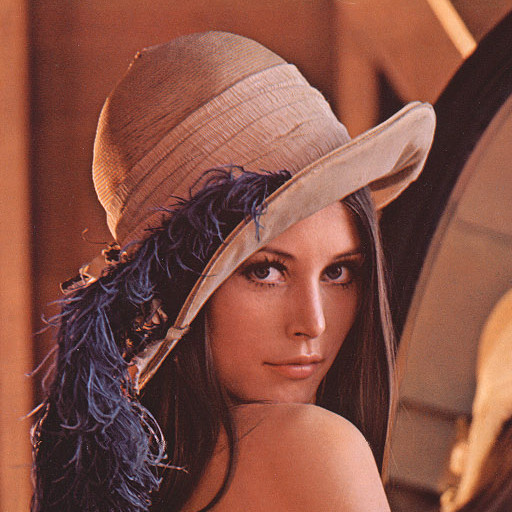
\includegraphics[width=7cm]{lena}};

  % Draw lines : input image -> input table
  \foreach \ref in {north west,north east,south west,south east}
    \draw[line] (lena.\ref) -- ++(\dx,\dy);

  % Draw input table
  \pgftransformcm{1}{0}{0}{1}{\pgfpoint{\dx}{\dy}}
  \node[table,fill=Cyan!50,minimum width=3*\celldim,minimum height=3*\celldim] at (0,0) {}; % Window
  \table{0}{(0,0)}{8}{8}{$2$,$7$,$4$,$1$,$8$,$3$,$0$,$3$,$7$,$8$,$2$,$5$,$3$,$8$,$6$,$1$,$0$,$2$,$4$,$6$,$1$,$4$,$7$,$1$,$0$,$2$,$5$,$8$,$3$,$6$,$1$,$9$,$4$,$7$,$2$,$5$,$0$,$1$,$4$,$6$,$5$,$8$,$4$,$2$,$9$,$4$,$1$,$2$,$1$,$7$,$3$,$8$,$4$,$0$,$5$,$9$,$1$,$4$,$2$,$6$,$7$,$3$,$8$,$0$}{LimeGreen!40}
  
  \begin{pgfonlayer}{next}
    % Draw filter kernel
    \pgftransformcm{1}{0}{0}{1}{\pgfpoint{\dx}{\dy}}
    \table{1}{(0,0)}{3}{3}{$\rfrac{1}{9}$,$\rfrac{1}{9}$,$\rfrac{1}{9}$,$\rfrac{1}{9}$,$\rfrac{1}{9}$,$\rfrac{1}{9}$,$\rfrac{1}{9}$,$\rfrac{1}{9}$,$\rfrac{1}{9}$}{RedOrange!40}

    % Draw output pixel lines
    \foreach \ref/\x/\y in {north west/1/1,north east/-1/1,south west/1/-1,south east/-1/-1}
      \draw[line] ($(table-1.\ref)$) -- ++(0.75*\dx+\x*\celldim,0.75*\dy-\y*\celldim);

    % Draw output table
    \pgftransformcm{1}{0}{0}{1}{\pgfpoint{0.75*\dx}{0.75*\dy}}
    \node[table,fill=RedOrange!55,minimum width=\celldim,minimum height=\celldim] at (\celldim,-\celldim) {}; % pixel
    \table{2}{(0,0)}{8}{8}{$3$,$3$,$3$,$3$,$3$,$3$,$2$,$1$,$3$,$4$,$4$,$4$,$4$,$4$,$4$,$2$,$2$,$3$,$5$,$4$,$5$,$4$,$5$,$3$,$2$,$3$,$5$,$4$,$4$,$3$,$4$,$3$,$3$,$4$,$5$,$4$,$4$,$3$,$4$,$3$,$4$,$5$,$5$,$4$,$4$,$3$,$4$,$3$,$3$,$4$,$5$,$5$,$5$,$5$,$4$,$3$,$1$,$2$,$3$,$3$,$3$,$3$,$3$,$2$}{Goldenrod!40}

    % Draw lines : output table -> output image
    \foreach \ref in {north west,north east,south west,south east}
      \draw[line] (table-2.\ref) -- ++(\dx,\dy);

    % Draw output image
    \pgftransformcm{1}{0}{0}{1}{\pgfpoint{\dx}{\dy}}
    \node[anchor=north west,inner sep=0pt] (lena-filtered) at (0,0) {
\includegraphics[width=7cm]{lena-filtered}};
  \end{pgfonlayer}

  % Draw lines : input table -> filter kernel
  \foreach \ref in {north west,north east,south west,south east}
    \draw[line] (table-1.\ref) -- ++(-\dx,-\dy);

  % Draw labels
  \node[above] at (table-0.north east) {\sffamily\Large input};
  \node[above] at (table-1.north east) {\sffamily\Large filter};
  \node[above] at (table-2.north east) {\sffamily\Large output};

\end{tikzpicture}
\caption{Representation of box filter.}
\label{fig:box-filter}
\end{figure}
